%%%%%%%%%%%%%%%%%%%%%%%%%%%%%%%%%%%%%%%%%%%%%%%%%%%%%%%%%%%%%%%%%%
%%%%%%%% ICML 2017 EXAMPLE LATEX SUBMISSION FILE %%%%%%%%%%%%%%%%%
%%%%%%%%%%%%%%%%%%%%%%%%%%%%%%%%%%%%%%%%%%%%%%%%%%%%%%%%%%%%%%%%%%

% Use the following line _only_ if you're still using LaTeX 2.09.
%\documentstyle[icml2017,epsf,natbib]{article}
% If you rely on Latex2e packages, like most moden people use this:
\documentclass{article}

% use Times
\usepackage{times}
% For figures
\usepackage{graphicx} % more modern
%\usepackage{epsfig} % less modern
\usepackage{subfigure} 

% For citations
\usepackage{natbib}
\usepackage{amsmath}
% For algorithms
\usepackage{algorithm}
\usepackage{algorithmic}
\usepackage{amssymb}
\usepackage{amsthm}

% As of 2011, we use the hyperref package to produce hyperlinks in the
% resulting PDF.  If this breaks your system, please commend out the
% following usepackage line and replace \usepackage{icml2017} with
% \usepackage[nohyperref]{icml2017} above.
\usepackage{hyperref}

% Packages hyperref and algorithmic misbehave sometimes.  We can fix
% this with the following command.
\newcommand{\theHalgorithm}{\arabic{algorithm}}
\newcommand{\infdiv}{D_{KL}\infdivx}


% Employ the following version of the ``usepackage'' statement for
% submitting the draft version of the paper for review.  This will set
% the note in the first column to ``Under review.  Do not distribute.''
%\usepackage{icml2017} 

% Employ this version of the ``usepackage'' statement after the paper has
% been accepted, when creating the final version.  This will set the
% note in the first column to ``Proceedings of the...''
\usepackage[accepted]{icml2017}


% The \icmltitle you define below is probably too long as a header.
% Therefore, a short form for the running title is supplied here:
\icmltitlerunning{Non linear Mixed Effects Models: Bridging the gap between Random Walk Metropolis and Variational Inference}

\begin{document} 

\twocolumn[
\icmltitle{Non linear Mixed Effects Models:\\
Bridging the gap between Independent Metropolis Hastings and Variational Inference}

% It is OKAY to include author information, even for blind
% submissions: the style file will automatically remove it for you
% unless you've provided the [accepted] option to the icml2017
% package.

% list of affiliations. the first argument should be a (short)
% identifier you will use later to specify author affiliations
% Academic affiliations should list Department, University, City, Region, Country
% Industry affiliations should list Company, City, Region, Country

% you can specify symbols, otherwise they are numbered in order
% ideally, you should not use this facility. affiliations will be numbered
% in order of appearance and this is the preferred way.
\icmlsetsymbol{equal}{*}

\begin{icmlauthorlist}
% \icmlauthor{Belhal Karimi}{to}
% \icmlauthor{Marc Lavielle}{to}
% \icmlauthor{Eric Moulines}{to}
\icmlauthor{Anonymous Authors}{to}
\end{icmlauthorlist}

\icmlaffiliation{to}{Ecole Polytechnique, Palaiseau, France}

\icmlcorrespondingauthor{Belhal Karimi}{belhal.karimi@polytechnique.fr}

% You may provide any keywords that you 
% find helpful for describing your paper; these are used to populate 
% the "keywords" metadata in the PDF but will not be shown in the document
\icmlkeywords{boring formatting information, machine learning, ICML}

\vskip 0.3in
]

% this must go after the closing bracket ] following \twocolumn[ ...

% This command actually creates the footnote in the first column
% listing the affiliations and the copyright notice.
% The command takes one argument, which is text to display at the start of the footnote.
% The \icmlEqualContribution command is standard text for equal contribution.
% Remove it (just {}) if you do not need this facility.

%\printAffiliationsAndNotice{}  % leave blank if no need to mention equal contribution


\begin{abstract} 
Variational inference and MCMC methods have been two popular methods in order to sample from a posterior distribution. Whereas the former extends the computation feasibility to higher dimension, the latter takes advantage of nice convergence properties to the exact posterior distribution. In this work we'll draw the parallel between a famous MCMC scheme called the Independent Metropolis Hastings and Variational inference. We'll explain our work on both Linear and Non-linear Gaussian cases. In the non linear case, a new proposal will be introduced motivated by a faster convergence of the Markov chain.
\end{abstract} 

\section{Introduction}

We consider a complete model (y,z) where the realizations of y are observed and z is the missing data. When the complete model $p(y,z,\theta)$ is parametric, the goal is to compute the maximum likelihood (ML) estimate of the parameter of this joint distribution.
\begin{equation}
\theta^{ML} = \arg\max \limits_{\theta} p(y,\theta)
\end{equation}
When the direct derivation of this expression is hard, several methods use the complete model to iteratively find the quantity of interest.
The EM algorithm has been the object of considerable interest since its presentation by Dempster, Laird and Rubin in 1977. It has been relatively effective in context of maximum likelihood estimation of parameters of incomplete model (unobserved or more). This algorithm is monotonic in likelihood making it a stable tool to work with.

Yet, when the quantity computed at the E-step involves infeasible computations, new methods have been developed in order to by-pass the issue. The stochastic EM algorithm \citep{diebolt} has been proposed in the context of mixture problem and involves splitting the E-step in a first simulation of the latent variables step and then a direct evaluation of the complete log model. A Robbins Monroe type approximation can be used to evaluate that latter quantity after the simulation step, that is the SAEM algorithm \citep{lavielle2,moulines}.


%-----------------------------------------------

\section{Model and notations}
We study a classical missing data problem where:
\begin{itemize}
\item The observed data is a continuous random variable $Y = (Y_i, 1\leq i \leq N)$ that has observed values $(y_i, 1\leq i \leq N)$ in $\mathcal{Y}$
\item The latent data is a continuous random variable $Z = (Z_i, 1\leq i \leq N)$ that takes on the values $(z_i, 1\leq i \leq N)$ in $\mathcal{Z}$ and consists in $N$ independent variables
\item The components $Y_i$ are generated independently of each other and from their corresponding $Z_i$
\item $\log p(y,\theta)$ is the incomplete data log-likelihood
\item $\log p(y,z,\theta)$ is the complete data log-likelihood and obtained by augmenting the observed data with the missing data
\item We'll call $P_{Y_i,Z_i,\theta}$ and $P_{Z_i|Y_i,\theta}$ the probability distributions associated to the densities $p(y_i,z_i,\theta)$ and $p(z_i|y_i,\theta)$
\end{itemize}


%------------------------------------------------

\section{Maximum likelihood estimation}
Our problem joins a familiar class of problem in computational statistics that consists in maximizing the following quantity:
\begin{equation}
\log p(y,\theta) = \int_{}{\log p(y,z,\theta)\mu(dz)}
\end{equation}
When this quantity can not be computed in closed form, many algorithms use iterative procedure to find the maximum likelihood parameter estimate. Among those techniques, the EM algorithm \citep{dempster}. This two steps algorithm consists in maximizing an auxiliary quantity that is the expectation of the complete log-likelihood with respect to the conditional distribution over the missing variable conditioned on the current parameter estimate (also called the posterior distribution).\\
Several alternatives have been developed throughout the past decades. Most of them alleviate the computation of the expectation using approximates. The MCEM algorithm \citep{diebolt} approximate this quantity by a Monte Carlo integration, the SAEM algorithm \citep{lavielle} uses a stochastic approximation of this quantity.\\

In those both cases, we need to be able to simulate from the posterior distribution $P(Z_i|Y_i,\theta)$. In most of the cases, this probability density function is intractable. As a result, variants include MCMC or Variational Inference engines to sample from this distribution. That's where we are focusing. In the sequel, the parameter $\theta$ is thus fixed to a certain value $\theta_0$ that will remains unchanged.\\

\section{Background on Posterior sampling} 
 
\subsection{Independent Metropolis Hastings}
Metropolis-Hastings are a powerful class of inference algorithms that belong to the family of  MCMC methods. This kind of algorithm constructs a Markov Chain by proposing candidate states sampled from a proposal distribution and then accepting or rejecting it according to the MH-step (see Algorithm ~\ref{alg:IMH} for detail). When this proposal is independent of the current state of the chain, we call the algorithm Independent Metropolis Hastings.

\begin{algorithm}[h]
   \caption{Independent Metropolis Hastings}
   \label{alg:IMH}
\begin{algorithmic}
   \STATE {\bfseries Input:} initial state $Z_0$, proposal distribution $q$, number of iterations $M$, target measure $\pi$


   \FOR{$m=1$ {\bfseries to} $M$}
   \STATE $Z_m \sim q(Z)$
   \STATE $\alpha(Z_m,Z_{m-1}) = \frac{\pi(Z_m) q(Z_{m-1})}{\pi(Z_{m-1}) q(Z_{m})}$
   \STATE Accept $Z_m$ with probability $\min(\alpha,1)$
   \ENDFOR

\end{algorithmic}
\end{algorithm}

We will explicitly write our target measure $\pi$ in the different cases we'll deal with in the sequel.\\

\subsection{Variational Inference}
Variational methods approximates those intractable distributions by finding the best distribution minimizing a divergence criteria. Let $\mathcal{D}$ be a family of distributions over the latent variable $Z_i$. Variational Methods solve the following optimization problem:
\begin{equation}
q^* = \arg \min \limits_{q \in \mathcal{D}} D_{KL}(q||P_{Z_i|Y_i,\theta_0})
\end{equation}

Which simplifies to:
\begin{equation}
q^* = \arg \max \limits_{q \in \mathcal{D}} \mathcal{L}(q)
\end{equation}
Where $\mathcal{L}(q) = \mathbb{E}_q(\log p(y_i,z_i,\theta_0)) - \mathbb{E}_q(\log q(z_i))$ is called the ELBO (Evidence Lower BOund).\\

The practical implementation of such an algorithm consisting in first, restricting the search space to a family of known distributions (in our case the Gaussian family). Then, performing a Monte Carlo integration of the gradient of the ELBO, see \citep{ranganath} and finally performing a gradient ascent  as described by Algorithm ~\ref{alg:VI}. We restrict ourselves to the family of Gaussian distributions of mean $\mu$ and variance $\Gamma$. We run the variational inference on the mean and fix the value of $\Gamma$. As a result the problem now is written, if we denote $q_{\mu}$ the Gaussian density of mean $\mu$:
\begin{equation}
\mu^* = \arg \max \limits_{\mu \in \mathbb{R}} \mathcal{L}(\mu)
\end{equation}

Where $\mathcal{L}(\mu) = \mathbb{E}_{q_{\mu}}(\log p(y_i,z_i,\theta_0)) - \mathbb{E}_{q_{\mu}}(\log q_{\mu}(z_i))$

\begin{algorithm}[h]
   \caption{Gradient Descent for VI}
   \label{alg:VI}
\begin{algorithmic}
   \STATE {\bfseries Input:} number of iterations $K$, initial $\mu_0$, stepsize $\rho$
  \STATE Initialize $\mu^0 = \mu_0$.
   \FOR{$k=1$ {\bfseries to} $K$}
   \STATE $\mu^k <- \mu^{k-1} + \rho \nabla_{\mu} \mathcal{L}$
   \ENDFOR
  \STATE Return $\mu^K$
\end{algorithmic}
\end{algorithm}


\section{Mixed effect models} 

In our domain of applications, mainly pharmacokinetic and pharmacodynamic (PK-PD) data analysis, we are mostly facing mixed effects models:

\begin{equation}
y_{ij} = f(\psi_i) + \epsilon_{ij}
\end{equation}

Where $f: \mathbb{R}^d \to \mathbb{R}$ is the structural model and is a function of $\psi_i$ that can be linear or not, $\psi_i \in \mathbb{R}^d$ are the individual parameters, $y_{ij}$ are the observations for individual i and $\epsilon_{ij} \sim \mathcal{N}(0,\Sigma)$. There can be more than one observation (subscript j) per individual. The parameters $\psi_i$ are composed of a fixed part $\psi_{pop}$ and a random one $\eta_i$:
\begin{equation}
\psi_i = \psi_{pop} + \eta_i 
\end{equation}
where $\eta_i \sim \mathcal{N}(0,\Omega)$.

In this context, our goal is to sample from the posterior $P(\psi_i|y_i,\theta_0)$ for all individuals. For simplicity we'll consider the centered random variable $\eta_i$ in our study. Thus, the goal is to sample from $P(\eta_i|y_i,\theta_0) = P(y_i|\eta_i,\theta_0)P(\eta_i)$. For the purpose of the stochastic EM algorithm we can easily shift to $\psi_i = M(\eta_i, \psi_{pop})$.\\
We'll now separate the cases where the structural model is linear or not and explain how MCMC are Variational Inference can be applied to our problem.

\subsection{Gaussian linear case}
For simplicity, we omit the number of observations per individual. The model can be written as:
\begin{equation}
y_{i} = A_i \psi_i + \epsilon_{i} 
\end{equation}
Where $A_i$ is a design matrix and $\psi_i = \psi_{pop} + \eta_i$. In this case, the true posterior is tractable and we can easily calculate that:
\begin{equation}
\eta_i|y_i \sim \mathcal{N}(m,G)
\end{equation}
Where $m = \Gamma A_i^\prime \Sigma^{-1} (y_i - A_i\psi_{pop})$ and $G = (A_i^\prime\Sigma^{-1}A_i + \Omega^{-1})^{-1}$

In this case, we can sample directly from the true posterior distribution. Thus, using MCMC or Variational Inference has no sense. We can verify that those both methods, whether we propose in the context of an MCMC with the true posterior or we apply a gradient descent over the mean of a candidate distribution, will converge to the right distribution.

\subsection{Gaussian non linear case}
The model can be written as:
\begin{equation}
y_{i} = f(\psi_i) + \epsilon_{i} 
\end{equation}
Where $f:\mathbb{R}^d \to \mathbb{R}$ is a non linear function and $\psi_i = \psi_{pop} + \eta_i$. The posterior distribution $P(\eta_i|y_i,\theta_0)$ is intractable in this case.\\
We are constructing a new independent proposal distribution for our Metropolis Hastings algorithm based on the linearization of this model around the maximum a posteriori (MAP) $\hat{\psi_i}$.
\begin{equation}
\hat{\psi_i} = \arg \max \limits_{\psi_i} P(\psi_i | y_i ; \theta_0)
\end{equation}
which can rewrite, considering the distribution of the components of the model:
\begin{equation}
\begin{split}
\hat{\psi_i}  = \arg \max \limits_{\psi_i} \quad & (y_i-f(\psi_i))' \Sigma^{-1} (y_i-f(\psi_i)) \\
&  + (\psi_i - \psi_{pop})' \Omega^{-1} (\psi_i - \psi_{pop})
\end{split}
\end{equation}

The Taylor expansion around this point gives the following expression:
\begin{equation}
y_{i} = f(\hat{\psi_i}) + \nabla_{\psi}f(\hat{\psi_i})(\psi_i - \hat{\psi_i}) + \epsilon_{i}
\end{equation}
Writing that $\psi_i = \psi_{pop} + \eta_i$ and developing the relation in order to have a linear expression in $\eta_i$, we obtain:
\begin{equation}
y_{i} - f(\hat{\psi_i}) - \nabla_{\psi}f(\hat{\psi_i})(\psi_{pop} - \hat{\psi_i}) = \nabla_{\psi}f(\hat{\psi_i})\eta_i + \epsilon_{i}
\end{equation}
We can now write the posterior distribution $\eta_i|y_i$ and show that  $\eta_i|y_i \sim \mathcal{N}(\mu_{lin},\Gamma_{lin})$ where
$\mu_{lin} = \mathbb{E}(\eta_i|y_i) = \hat{\eta_i} = \hat{\psi_i} - \psi_{pop}$ and $\Gamma_{lin}^{-1} = \nabla_{\psi}f(\hat{\psi_i})'\Sigma^{-1} \nabla_{\psi}f(\hat{\psi_i}) + \Omega^{-1}$ 

This new distribution will serve as an independent (independent of the current state of the chain since always centered in $\hat{\eta_i}$) proposal for our MH algorithm.\\
The other aspect we want to develop is to know if a variational approach where our candidate distribution would be taken in the family of the Gaussian distributions with variance $\Gamma_{lin}$ and with mean $\mu$ on which we'll do perform the gradient ascent, would converge to the same mean $\hat{\eta_i}$. In other words, we want to highlight the equivalence of those two methods based on the same approximation (that the proposal is a Gaussian distribution even though, due to the non-linearity of the model, the true posterior does not belong to a known family of distribution).

\section{Experiments} 

\subsection{One-compartment model for Theophylline}
This section develops the application of those two methods on a Pharmacokinetics (PK) example. Beforehand, the standard approach is to approximate the body as a simple compartment models. In this example we will focus on a one-compartment model for theophylline following oral dose D at time $t=0$ leading to description of concentration $y(t_i)$ at time $t_i \geq 0$ (i varies from 1 to N and denote the individual of the population):
\begin{equation}
y_i = y(t_i) = f(\psi_i)+ \epsilon_i
\end{equation}
With :
\begin{equation}
f(\psi_i) = \frac{D(k_a)_i}{V_i((k_a)_i - (C_l)_i/V_i)}(e^{(-(k_a)_it_i)}-e^{(-\frac{(C_l)_i}{V_i}t_i)})
\end{equation}
Where $(k_a)_i$ is the fractional rate of absorption for individual $i$, $(C_l)_i$ is the clearance rate for individual $i$ and $V_i$ is the volume of distribution for individual $i$ and D is the dose injected.\\
In our notation, the complete model is $p(y_i,\psi_i,\theta_0)$ where $\psi_i = ((k_a)_i, (C_l)_i, V_i)$ is the vector of individual parameters where each component is composed of a fixed effect term and a random effect (a centered Gaussian with same variance $\Omega$) and $\theta_0 = (\Omega_0, \Sigma_0$ (with $\epsilon_i \sim \mathcal{N}(0,\Sigma_0)$ and $(k_a)_i = (k_a)_{pop} + \eta_{(k_a)_i}$ and $\eta_{(k_a)_i} \sim \mathcal{N}(0,\Omega_0)$).\\
Our goal is to simulate for instance from the posterior distribution $P((k_a)_i|y_i,\theta_0)$. As we said above we can work on the distribution $P(\eta_{(k_a)_i}|y_i,\theta_0)$ and equivalently for the others parameters.\\
Following the method of linearization of this model as described above, we obtain faster convergence of the MH algorithm with this new independent proposal than our reference Random Walk Metropolis consisting in three successive kernels proposing with a Gaussian centered in the current state of the chain and whose variance adapts with respect to the optimum acceptance rate.

\begin{figure}[ht]
\vskip 0.2in
\begin{center}
\centerline{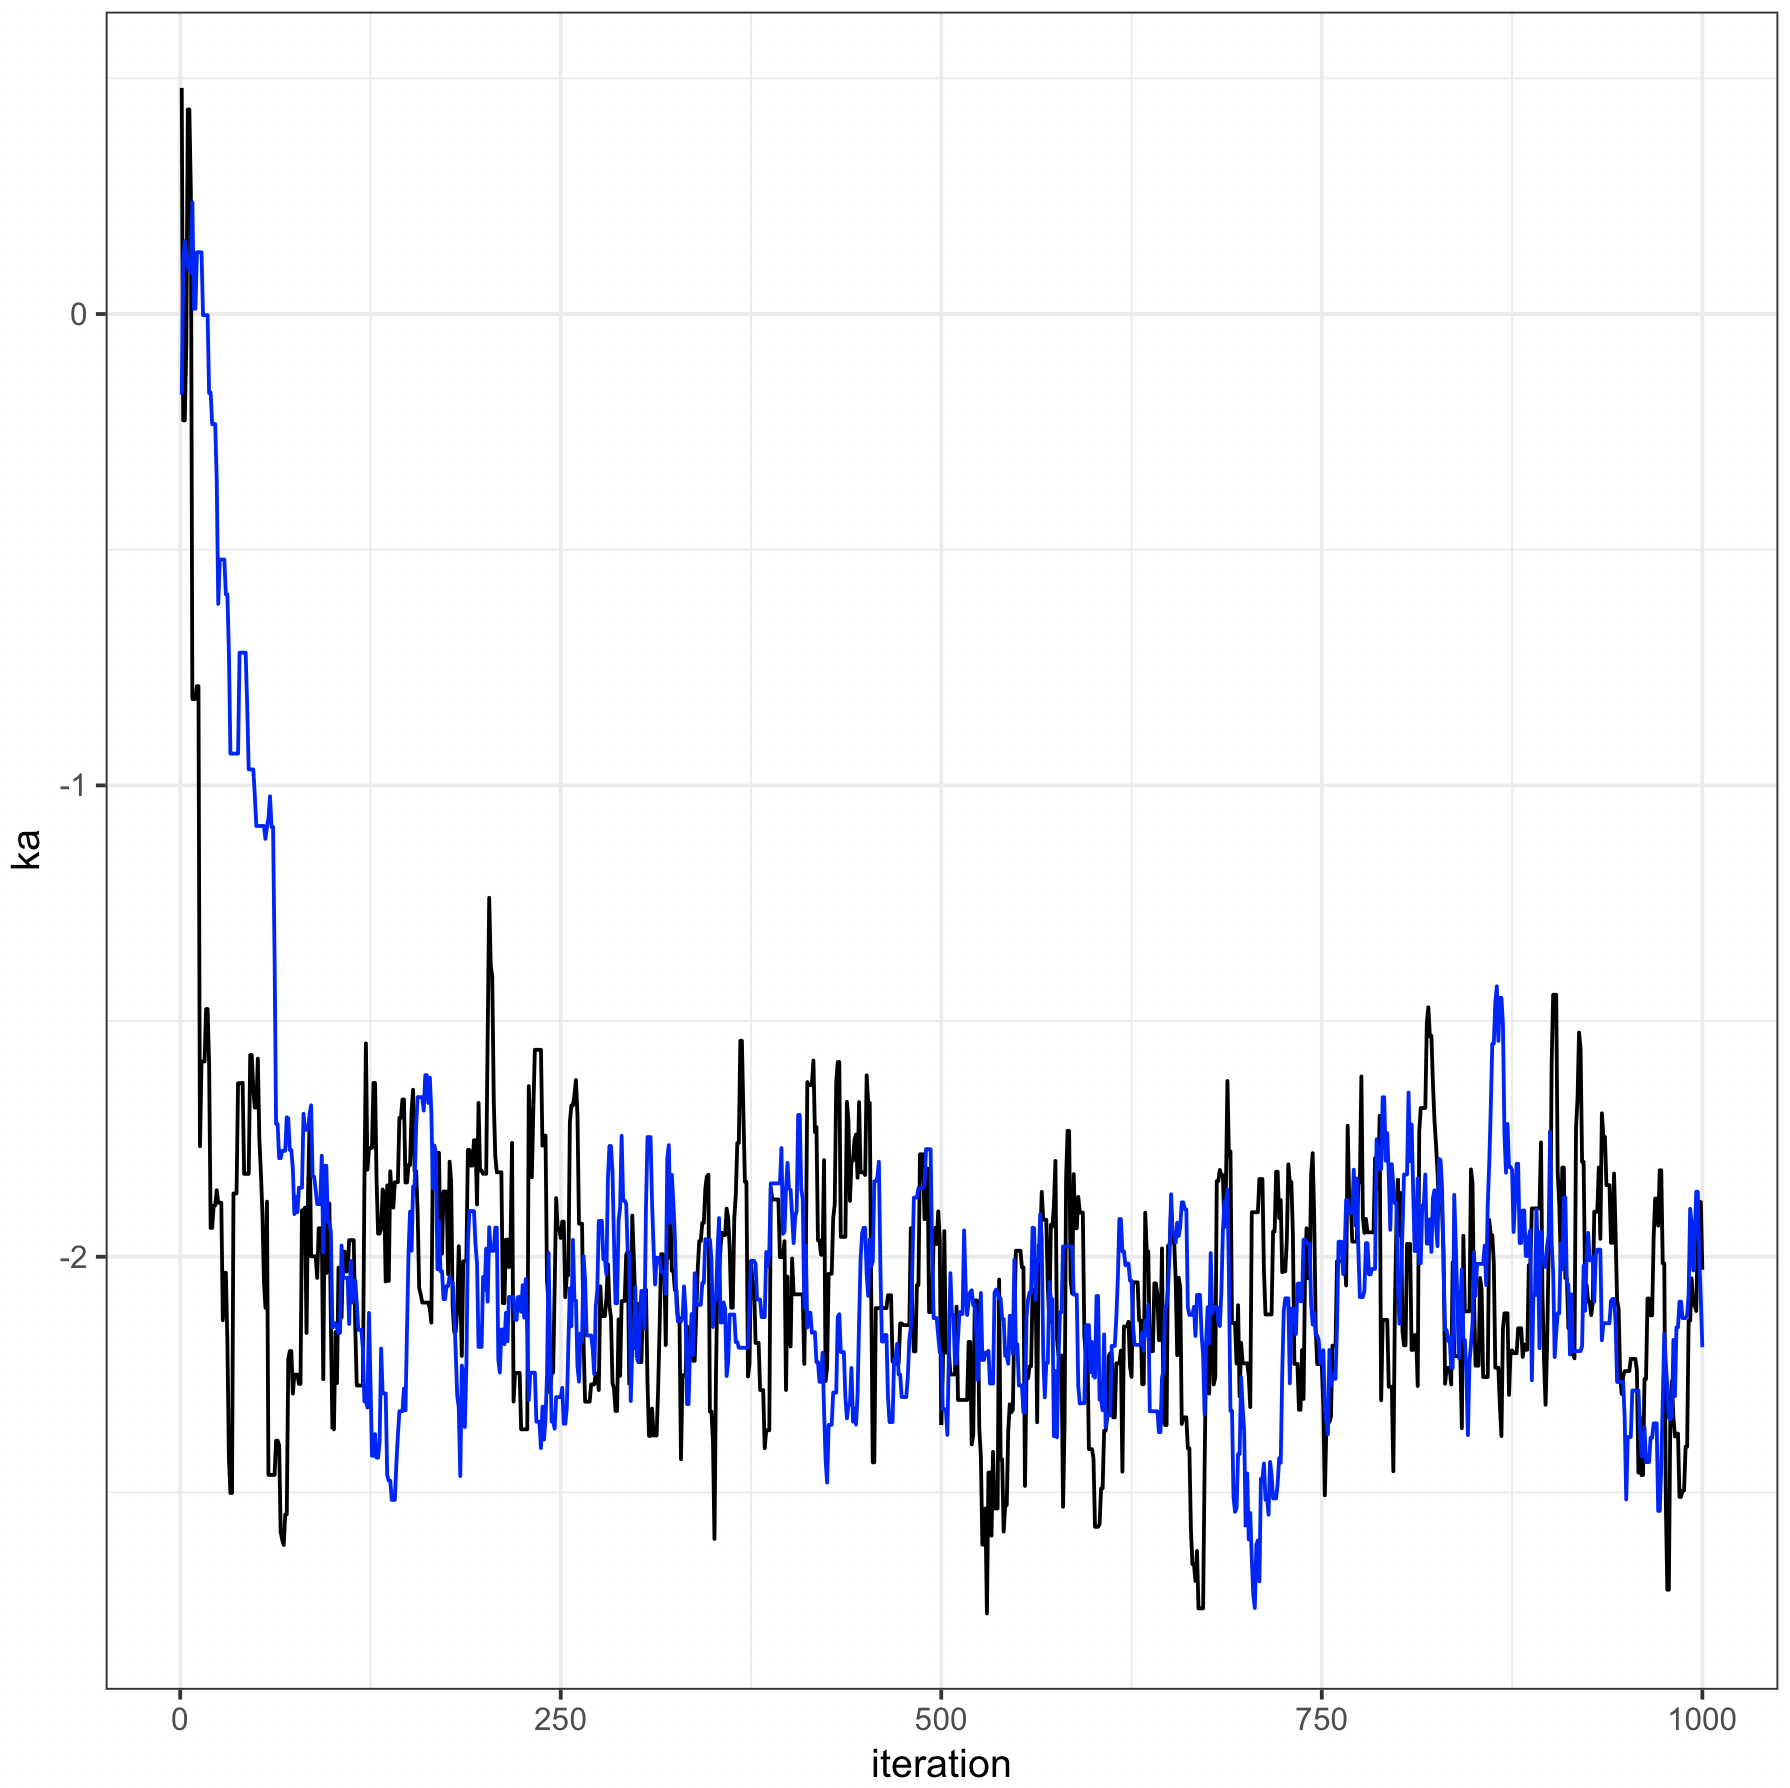
\includegraphics[width=\columnwidth]{new_kernel.png}}
\caption{MCMC samples. RWM in blue and Independent MH with our new proposal in black. 1000 iterations of MCMC iterations. Plotting the posterior distribution $P(\eta_{(k_a)_i}|y_i,\theta_0)$ for a random individual $i$}
\label{new}
\end{center}
\vskip -0.2in
\end{figure} 

\section{Discussion} 
This work is still in progress. Our goals are multiple. First of all, following \citep{kuhn} setting convergence properties for the SAEM algorithm coupled with an MCMC procedure, we are aiming at setting up similar properties for the SAEM coupled with a variational inference procedure (See also \citep{gunawardana} for the Variational EM algorithm). Moreover, we would like to theoretically draw some parallels between those two methods. And finally, many PK-PD models consider not continuous but categorical or count data. In this case, an alternative to linearization has to be found in order to construct such a proposal.\\
Also, in our context of applying this method to the SAEM algorithm, while calculating the MAP once for one MCMC run is not costly, doing it K times (K being the number of SAEM iterations) can be. We are investigating a way to calculate the MAP once at the beginning and then apply a single step of gradient descent at each SAEM iteration in order to slowly move the MAP estimate after each update of the posterior distribution towards a better approximation.
% In the unusual situation where you want a paper to appear in the
% references without citing it in the main text, use \nocite

\bibliography{example_paper}
\bibliographystyle{icml2017}

\end{document} 


% This document was modified from the file originally made available by
% Pat Langley and Andrea Danyluk for ICML-2K. This version was
% created by Lise Getoor and Tobias Scheffer, it was slightly modified  
% from the 2010 version by Thorsten Joachims & Johannes Fuernkranz, 
% slightly modified from the 2009 version by Kiri Wagstaff and 
% Sam Roweis's 2008 version, which is slightly modified from 
% Prasad Tadepalli's 2007 version which is a lightly 
% changed version of the previous year's version by Andrew Moore, 
% which was in turn edited from those of Kristian Kersting and 
% Codrina Lauth. Alex Smola contributed to the algorithmic style files.  
